\documentclass[11pt]{report}
% this template is originally from Roy Dong's ECE 515.
% Edited by Dawei Sun
%%%%%%%%%%%%%%%%%%%%%%%%%%%%%%%%%%%%%%%%%%%%%%%%%%%%%%%%%%%%%%%%%%
% Set the margins of our document.
\usepackage[margin = 1 in]{geometry}

%%%%%%%%%%%%%%%%%%%%%%%%%%%%%%%%%%%%%%%%%%%%%%%%%%%%%%%%%%%%%%%%%%
% Import commands for custom header.
\usepackage{fancyhdr}
\pagestyle{fancy}

%%%%%%%%%%%%%%%%%%%%%%%%%%%%%%%%%%%%%%%%%%%%%%%%%%%%%%%%%%%%%%%%%%
% Allow ourselves to do equations!
\usepackage{amsmath,amssymb,amsthm,amsfonts}
\usepackage{upgreek}
\usepackage{mathtools}
\usepackage{bbm}

%%%%%%%%%%%%%%%%%%%%%%%%%%%%%%%%%%%%%%%%%%%%%%%%%%%%%%%%%%%%%%%%%%
% Nicer formatting for enumerate commands.
\usepackage[shortlabels]{enumitem}

\usepackage{algorithm2e}
\usepackage[noend]{algpseudocode}

%%%%%%%%%%%%%%%%%%%%%%%%%%%%%%%%%%%%%%%%%%%%%%%%%%%%%%%%%%%%%%%%%%
% Colored text and include images.
\usepackage{color}
\usepackage[dvipsnames]{xcolor}
\usepackage{graphicx}

\usepackage{listings}
\usepackage{multicol}
%%%%%%%%%%%%%%%%%%%%%%%%%%%%%%%%%%%%%%%%%%%%%%%%%%%%%%%%%%%%%%%%%%
% Some custom macros to make life easier.
\newcommand{\mc}{\mathcal}
\newcommand{\mb}{\mathbb}
\newcommand{\reals}{\mathbb{R}}

\newcommand{\T}{\intercal}
\newcommand{\E}[1]{\mathbb{E}\left[#1\right]}

%%%%%%%%%%%%%%%%%%%%%%%%%%%%%%%%%%%%%%%%%%%%%%%%%%%%%%%%%%%%%%%%%%
%%%%%%%%%%%%%%%%%%%%%%%%%%%%%%%%%%%%%%%%%%%%%%%%%%%%%%%%%%%%%%%%%%
%%%%%%%%%%%%%%%%%%%%%%%%%%%%%%%%%%%%%%%%%%%%%%%%%%%%%%%%%%%%%%%%%%

\lhead{ECE 553 - Fall 2020 at University of Illinois at Urbana-Champaign}
\rhead{\textcolor{red}{Dawei Sun (daweis2)}}

%%%%%%%%%%%%%%%%%%%%%%%%%%%%%%%%%%%%%%%%%%%%%%%%%%%%%%%%%%%%%%%%%%
%%%%%%%%%%%%%%%%%%%%%%%%%%%%%%%%%%%%%%%%%%%%%%%%%%%%%%%%%%%%%%%%%%
%%%%%%%%%%%%%%%%%%%%%%%%%%%%%%%%%%%%%%%%%%%%%%%%%%%%%%%%%%%%%%%%%%

\begin{document}

%%%%%%%%%%%%%%%%%%%%%%%%%%%%%%%%%%%%%%%%%%%%%%%%%%%%%%%%%%%%%%%%%%
%%%%%%%%%%%%%%%%%%%%%%%%%%%%%%%%%%%%%%%%%%%%%%%%%%%%%%%%%%%%%%%%%%
%%%%%%%%%%%%%%%%%%%%%%%%%%%%%%%%%%%%%%%%%%%%%%%%%%%%%%%%%%%%%%%%%%

\section*{Exercise 4.1}
Let $x=[x_1, x_2]$, $p=[p_1, p_2]$, $u = [u_1, u_2]$. We have that $H = (p_1 u_1 + p_2 u_2)\sqrt{x_2} + p_0$. From here onward, the expressions are evaluated along the optimum, and we omit the $*$. Let $u_1 = \cos(\theta)$ and $u_2 = \sin(\theta)$. According to the maximum principle, $H_{\theta} = \sqrt{x_2}(-p_1 \sin(\theta)+p_2\cos(\theta)) = 0$. Thus, $\tan(\theta) = p_2/p_1$. Thus, we have $u_1 = \frac{p_1}{\|p\|}$ and $u_2 = \frac{p_2}{\|p\|}$. Moreover, $\dot{p}_1 = -H_{x_1} = 0$, $\dot{p}_2 = -H_{x_2} = -\|p\| \frac{1}{2\sqrt{x_2}}$. Clearly, $p_1$ is a constant. Now, consider the derivatives of $x_2$ w.r.t. $x_1$. First, $\frac{dx_2}{dx_1} = \frac{\dot{x}_2}{\dot{x}_1} = \frac{p_2}{p_1}$. Second, $\frac{d^2 x_2}{dx_1^2} = \frac{1}{p_2} \cdot \frac{dp_2}{dx_1} = \frac{1}{p_1} \cdot \frac{\dot{p}_2}{\dot{x}_1} = -\frac{\|p\|^2}{2p_1^2 x_2}$. Now, consider the optimal curve $x_2(x_1)$, then we have that $1+x_2'^2+2x_2x_2''=0$, which gives cycloids.

% \section*{Exercise 4.2}
% Hello Guilherme,

% \noindent This is a placeholder. Please grade this one with score $0$. For this homework, I choose $L=3$ and $R=1$. I will resubmit this one after the graded homework is returned. Late submissions: $\{4.5, 4.7, 4.8\}$. Resubmissions: $\{4.2\}$. This configuration is indeed the same as $L=4$ and $R=0$. But I noticed that $L$ and $R$ have to be positive integers. Thank you.

\section*{Exercise 4.3}
Since $x^0$ does not appear in the RHS of the dynamics of the augmented system, it is clear that if $y$ is a valid trajectory, translating $y$ along the $x^0$-axis also gives a valid trajectory. If we can find a trajectory from $t_1$ to $t_3$ such that it reaches $S''$ below the optimal trajectory, then we can shift the $[t_2, t^*]$ part of the optimal trajectory downward to connect it with the newly found trajectory at $S''$. Then, shift the time variable accordingly (we can do that since the dynamics and the running cost are both time-invariant), and the resulting terminal time is still greater than $t_0$ and thus valid. Then, we get a new trajectory which reaches $S'$ below the optimal one, which is not possible.

\section*{Exercise 4.4}
Lets translate $I_1$ a little bit: $\tilde{I}_1 = (b-\epsilon (a_1+a_2), b-\epsilon a_2]$. The perturbed control is
\[u(t) = \begin{cases} w_1 & \mbox{if } t \in \tilde{I}_1,\\ w_2 & \mbox{if } t \in I_2,\\ u^*(t) & \mbox{otherwise}.\end{cases}\]
Then, we have
\begin{align^*}
y\left(t^{*}\right) &=y^{*}\left(t^{*}\right)+\varepsilon \Phi_{*}\left(t^{*}, {b-a_2\varepsilon}\right) \nu_{b-a_2\varepsilon}\left(w_{1}\right) a_{1}+\varepsilon \delta\left(w_{2}, I_{2}\right)+o(\varepsilon).
\end{align^*}
From the definition of $\nu$ and the fact that $g$ is smooth, we know $\nu_{b-a_2\varepsilon}\left(w_{1}\right) = \nu_{b}\left(w_{1}\right) + O(\varepsilon)$, where $O(\varepsilon)$ is an infinitesimal quantity of the same order as $\varepsilon$. Similarly, $\Phi_{*}\left(t^{*}, {b-a_2\varepsilon}\right) = \Phi_{*}\left(t^{*}, {b}\right) + O(\varepsilon)$. Thus, $\varepsilon \Phi_{*}\left(t^{*}, {b-a_2\varepsilon}\right) \nu_{b-a_2\varepsilon}\left(w_{1}\right) a_{1} = \varepsilon \delta\left(w_1, I_1) + o(\varepsilon)$.

Actually, there could even be a gap between $\tilde{I}_1$ and $I_2$, but as long as the length of this gap is of higher or the same order as $\epsilon$, we can get the desired change on the terminal state. This fact may be helpful when generalizing this result to more than two intervals.
\section*{Exercise 4.6}
Next, we prove that the limits of the LHS and RHS of (4.36) divided by $(t-t')$ are zero. For any nearby $t$ and $t'$, expanding the first term of the LHS at $t$ gives
\begin{multline*}
H\left(x^{*}\left(t^{\prime}\right), u^{*}(t), p^{*}\left(t^{\prime}\right), p_{0}^{*}\right)-H\left(x^{*}(t), u^{*}(t), p^{*}(t), p_{0}^{*}\right) \\= (H_x\left(x^{*}(t), u^{*}(t), p^{*}(t), p_{0}^{*}\right) \dot{x}^* + H_p\left(x^{*}(t), u^{*}(t), p^{*}(t), p_{0}^{*}\right) \dot{p}^*)(t^{\prime}-t) + o(t^{\prime}-t) \\= (-\dot{p}^{*}\dot{x}^* + \dot{x}^*\dot{p}^*)(t^{\prime}-t) + o(t^{\prime}-t) = o(t^{\prime}-t).
\end{multline*}
Thus, $\lim_{t^{\prime} \to t} = \frac{LHS}{t-t^{\prime}} = 0$. Similarly, expanding the second term of the RHS at $t^{\prime}$ gives $\lim_{t^{\prime} \to t} \frac{RHS}{t-t^{\prime}} = 0$. Thus, $\lim_{t^{\prime} \to t} \frac{m - m'}{t-t^{\prime}} = 0$.

\section*{Exercise 4.7}
Let $p_0^* = -1$, then we have
\begin{equation}
\dot{p}^* = \dot{\bar{p}}^{*} - \left.K_{x x}\right|_{*} f\right|_{*} = -\left.\left(f_{x}\right)^{T}\right|_{*} \bar{p}^{*}+\left.\left(f_{x}\right)^{T}\right|_{*} \left. K_{x}\right|_{*} = -\left.\left(f_{x}\right)^{T}\right|_{*}(\bar{p}^{*} - \left.K_{x}\right|_{*}) = -\left.\left(f_{x}\right)^{T}\right|_{*} p^* = -\left.H_x\right|_*.
\end{equation}

\noindent Since we have $\dot{p}^* = -\left.\left(f_{x}\right)^{T}\right|_{*} p^*$, $p^*(t) = 0$ for some $t$ implies $p^*(t) \equiv 0$, which contradicts the fact that $p^*(t^*) = -K_x(x^*(t^*)) \neq 0$.

% \section*{Exercise 4.8}

\section*{Exercise 4.9}
For the case where $y^*(t_0)$ is fixed, we denote by $C_{t^*}$ the cone resulted by the admissible perturbations. Also, $C_{t^*}$ lies in the negative side of the plane determined by the normal $\begin{pmatrix}p^*_0\\p^*(t^*)\end{pmatrix}$. Now considering the system running backward in time, fixed the initial state $y^*(t^*)$, the cone resulted by admissible perturbations is denoted by $-C_{t_0}$. Intuitively, we can interpret $-C_{t_0}$ as follows. Considering the original system, $-C_{t_0}$ can be viewed as a initial set such that starting from any element in $-C_{t_0}$, we can find an admissible perturbation such that the terminal state $y^*(t^*)$ does not change compared to that starting from $y^*(t_0)$, i.e. the perturbation on the initial state can be canceled by the perturbation on the control. Furthermore, from Eq. 4.32 in the textbook, we know that $-C_{t_0}$ exactly lies in the {\em positive} side of the plane determined by the normal $\begin{pmatrix}p^*_0\\p^*(0)\end{pmatrix}$.

Considering the following set
\begin{equation}
T:=\left\{y \in \mathbb{R}^{2n+2}: y=\left(\begin{array}{l}y^{*}(0)\\y^{*}(t^*)\end{array}\right)+\left(\begin{array}{l}0\\d_1\\0\\d_2\end{array}\right)+\beta \left(\begin{array}{l}0\\\mu\end{array}\right), d_1 \in T_{x^{*}\left(t_0\right)} S_{t_0}, d_2 \in T_{x^{*}\left(t^*\right)} S_{t^*}, \beta \geq 0\right\},
\end{equation}
we must have that $T$ and $-C_{t_0} \bigotimes C_{t^*}$ are disjoint. Otherwise, we can find admissible perturbations with new admissible initial and terminal states such that the cost is reduced. Let $\beta=0$, we get that $\left\langle \left(\begin{array}{l}-p^*(0)\\p^{*}(t^*)\end{array}\right), d \right\rangle \geq 0$. We add ``$-$" to $p^*(0)$ because $-C_{t_0}$ lies in the {\em positive} side of the plane and $T$ has to lie in the negative side. Since the tangent space is closed under negation, we must have that $\left\langle \left(\begin{array}{l}-p^*(0)\\p^{*}(t^*)\end{array}\right), d \right\rangle = 0$.

\section*{Exercise 4.10}
In this case, $S_1$ is not a single-point set. Using the transversality condition, we know that $p_1^*(t^*) = 0$. Since $p_1^*$ is a constant function, it immediately follows that $p_1^* \equiv 0$. Thus, $p_2^*$ is a nonzero constant function without any zero crossings. Everything else in the previous derivation remains the same. Thus, the optimal control is bang-bang type but without switching. Instead, $u^*$ is either $1$ or $-1$ constantly for all $t$. Using Fig. 4.15, we know that if $x(0) < 0$ (starts from the left half of the $x$-$\dot{x}$ plane), we set $u^* \equiv 1$, otherwise we set $u^* \equiv -1$.

\section*{Exercise 4.11}
The state equation of the system is
\begin{align*}
& \dot{x}_1 = x_2\\
& \dot{x}_2 = -x_1 + u.
\end{align*}
The Hamiltonian is $H = p_1 x_2 + p_2 (-x_1 + u) + p_0$. The optimal control $u^*$ is still the same as shown in Eq. 4.50, i.e. it is a bang-bang type control.

\noindent Furthermore, we have that $\dot{p}^*_1 = -H_{x_1} = -p^*_2$ and $\dot{p}^*_2 = -H_{x_2} = p^*_1$. Thus, $\ddot{p}_2^* + p_2 = 0$, which gives $p_2^* = c_1 \sin(t) + c_2 \cos(t)$. Thus, switching interval of $u^* = sgn(p_2^*)$ is $\pi$.

\noindent Since $x_2\dot{x}_2 + (x_1-u)\dot{x}_1 = 0$, we know that if $u$ is a constant, the trajectory curve is $(x_1-u)^2 + x_2^2 = r^2$ ($r \geq 0$), i.e. the system moves on the circle centered at $(u, 0)$. Consider a point $(x_1, x_2)$ on the circle such that $x_1 > u$ and $x_2 > 0$, we have that $\dot{x}_1 > 0$, which implies that the system moves in the clockwise direction on the circle. Moreover, the relationship between $x_1-u$ and $x_2$ is exactly the same as that between $p_1^*$ and $p^*_2$. Thus, the trajectory curve has the same period as the costate, which is $2\pi$. This implies that the system can travel a semi-circle between two switchings.

\noindent As shown in Figure~\ref{fig:411}, we have to control the system to the two thick curves which can drive the system to the origin without switching. Starting from the these thick curves, running the system backward in time, and considering the constraint that the trajectory between two switchings is a semi-circle., we arrive at the following control strategy. In the green region we set $u=-1$, and the system moves in the clockwise direction on the circle centered at $(-1,0)$. Similarly, in the red region, we set $u=1$. It is clear that the trajectory will finally hit the thick curves no matter where it starts.
\begin{figure}
    \centering
    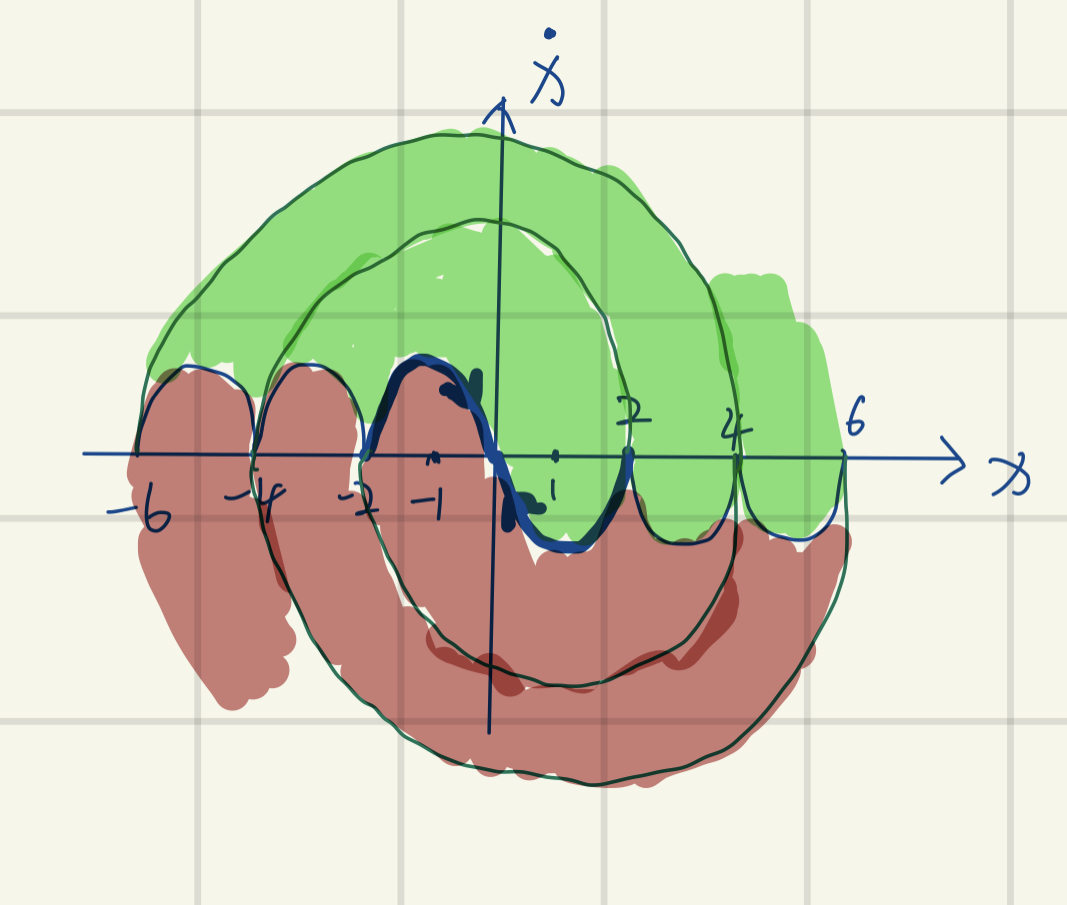
\includegraphics[width=.5\textwidth]{ECE553/hw5/hw5_411.jpg}
    \caption{Trajectories}
    \label{fig:411}
\end{figure}

\end{document}
